

\documentclass[a4paper]{article}

\usepackage{amsmath}
\usepackage{hyperref}
\usepackage{biblatex}
\usepackage{enumerate}
\usepackage{graphicx}
\usepackage{stmaryrd}
\usepackage[dvipsnames]{xcolor}
\usepackage{listings}
\usepackage{caption}
\usepackage{subcaption}
\usepackage{booktabs}


\addbibresource{refs.bib}

\begin{document}

\author{Ola Bratt \\
  \href{mailto:ola.bratt@gmail.com}{ola.bratt@gmail.com}
  \and
  Patrick Attimont \\
  \href{patrickattimont@gmail.com}{patrickattimont@gmail.com}
}

\title{DAT565/DIT407 Assignment 3}
\date{2024-02-xx}

\maketitle

This paper is addressing the assignment 3 study queries within the \emph{Introduction to Data Science \& AI} course, DIT407 at 
the University of Gothenburg and DAT565 at Chalmers. The main source of information for this project
is derived from the lectures and Skiena~\cite{Skiena:2024}. Assignment 3 is about text classification and the 
use of correct data splitting and encoding handling.

\section*{Problem 1: Spam and Ham}

\subsection*{A. Data exploration}
Spam is often recognizable for a human being as advertising a product.
Spam emails will often use hyperbolic adjectives to showcase or promote something, as well as links to different websites.
The end of the email could also be important to identify spam: it usually contains a paragraph stating that the user is subscribed to an email program with a link to unsubscribe.
This is an easily recognizable pattern for the classifier since it often uses the same words.

Hard ham seems to be closer to spam as it contains promotion emails and newsletter from websites and companies the user has subscribed to.
Therefore it can be more difficult for the classifier to separate the different emails.

\subsection*{B. Data splitting}
Since we have a large dataset, we can use the \texttt{train\_test\_split} function from the \texttt{sklearn.model\_selection}. With a smaller
dataset it would be better to use cross-validation to avoid overfitting.

\begin{verbatim}
  X_train, X_test, y_train, y_test = 
  train_test_split(email_matrix, labels, test_size=0.2)
\end{verbatim}
\section*{Problem 2: Preprocessing}
The "bag of words" model is a basic and intuitive way to analyze and compare documents based on their textual content. 
However, it does not consider the context or the order of words, which can limit its effectiveness in capturing the semantics 
and meaning of the text.
\section*{Problem 3: Easy Ham}

To calculate the precision, recall, accuracy and confusion matrix, we use the following code (These functions are available in the \texttt{sklearn.metrics} package): 
\begin{verbatim}
  accuracy = accuracy_score(y_test, y_pred)
  precision = precision_score(y_test, y_pred)
  recall = recall_score(y_test, y_pred)
  conf_matrix = confusion_matrix(y_test, y_pred)
\end{verbatim}

Accuracy measure the proportion of true results among the total number of cases examined, this is calculated according to Equation~\ref{equation:accuracy}. 
Precision measures the proportion of true positive results among the total number of cases that were predicted to be positive, this is calculated according to Equation~\ref{equation:precision}. 
Recall measures the proportion of true positive results among the total number of cases that were actually positive, this is calculated according to Equation~\ref{equation:recall}.
F1 score is the harmonic mean of precision and recall, this is calculated according to Equation~\ref{equation:f1}.
These metrics are used to evaluate the performance of the models. 
Valuse close to 1 indicates that a high percentage of the classifier's predictions are correct. 

The accuracy, precision, recall, and F1 score for the easy ham and spam dataset are shown in Table~\ref{tabular:easy_summary}. 
The confusion matrixes for the easy ham and spam dataset are shown in Figure~\ref{fig:easy_ham_and_spam_confusion_matrix}.
\begin{equation}
  \label{equation:accuracy}
  Accuracy =  \cfrac{ TP + TN}{TP + TN + FP + FN}  
\end{equation}
\begin{equation}
  \label{equation:precision}
  Precision = \cfrac{ TP}{TP + FP}  \\
\end{equation}
\begin{equation}
  \label{equation:recall}
  Recall = \cfrac{ TP}{TP + FN}  \\
\end{equation}
\begin{equation}
  \label{equation:f1}
  F1 = 2 * \cfrac{ Precision * Recall}{Precision + Recall}
\end{equation}

\begin{table}
  \begin{center}
  \begin{tabular}{ l|l|l|l|l }
    \hline
    \text{Model} & \text{accuracy} & \text{precision} & \text{recall} & \text{F1 score}\\
    \hline
    \text{Multinomial Naive Bayes} & 0.985 & 0.984 & 0.998 & 0.991 \\
    \text{Bernoulli Naive Bayes} & 0.923 & 0.918 & 0.996 & 0.956 \\
  \end{tabular}
\end{center}
\caption{Metrics for Easy Ham and Spam}
  \label{tabular:easy_summary}
\end{table}


\begin{figure}
  \centering
  \begin{subfigure}[a]{\textwidth}
      \centering
      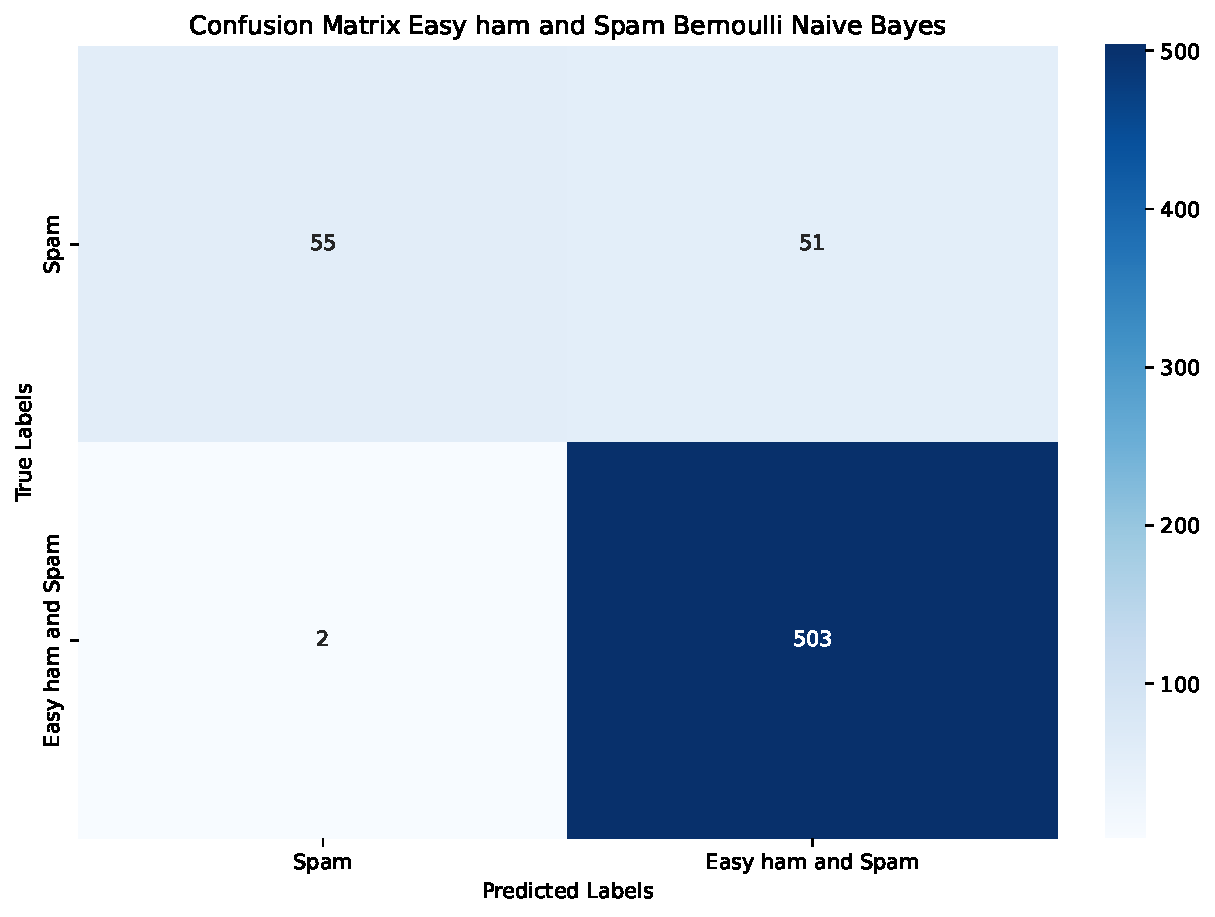
\includegraphics[width=\textwidth]{easy_ham_and_spam_bernoulli_naive_bayes_confusion_matrix.pdf}
      \caption{Easy ham vs spam, Bernoulli Naive Bayes}
      \label{fig:easy_ham_and_spam_bernoulli_naive_bayes_confusion_matrix}
  \end{subfigure}
  \vfill
  \begin{subfigure}[b]{\textwidth}
      \centering
      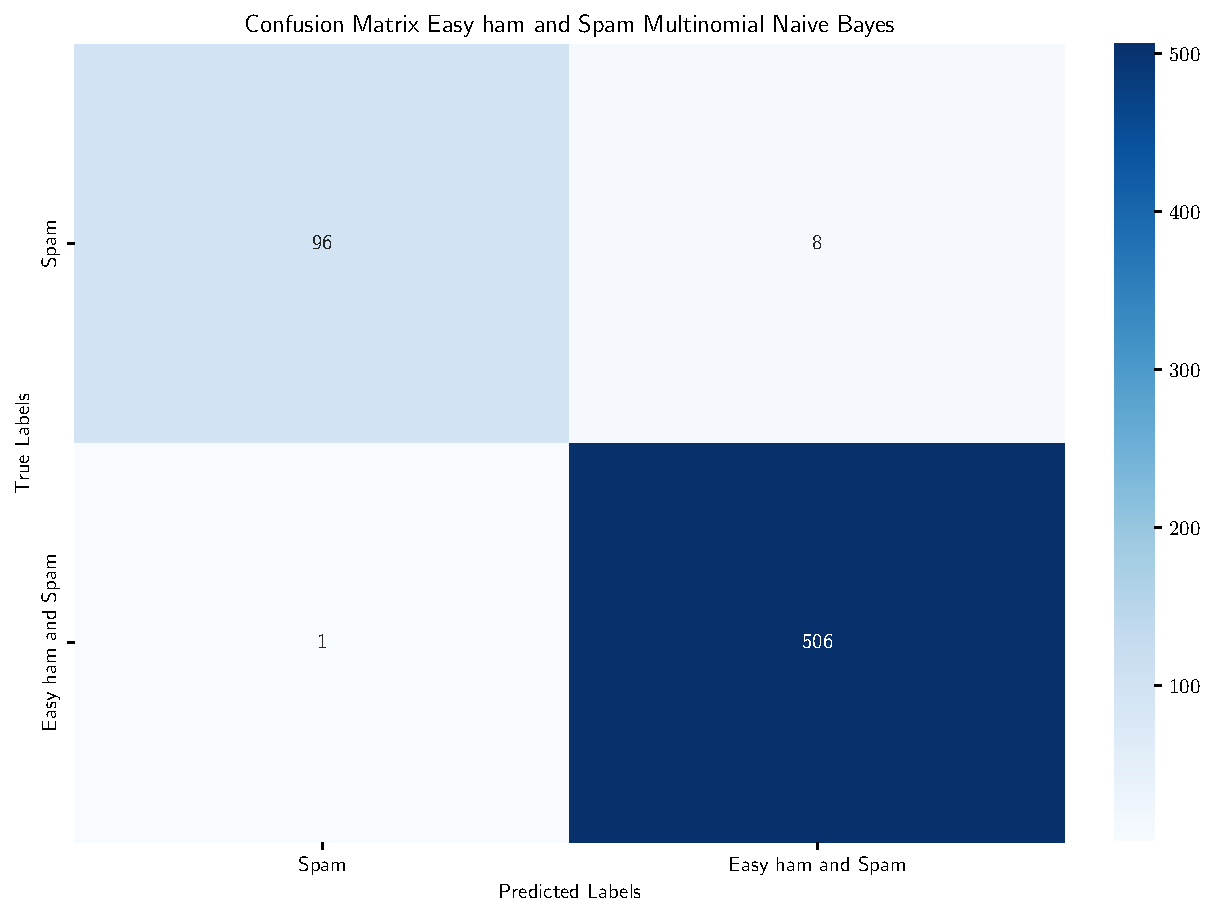
\includegraphics[width=\textwidth]{easy_ham_and_spam_multinomial_naive_bayes_confusion_matrix.pdf}
      \caption{Easy ham vs spam, Multinomial Naive Bayes}
      \label{fig:easy_ham_and_spam_multinomial_naive_bayes_confusion_matrix}
  \end{subfigure}
  \caption{Confusion matrixes of easy ham and spam}
  \label{fig:easy_ham_and_spam_confusion_matrix}
\end{figure}

\newpage
\section*{Problem 3: Hard Ham}
The accuracy, precision, recall, and F1 score for the hard ham and spam dataset are shown in Table~\ref{tabular:hard_summary}.
The confusion matrixes for the hard ham and spam dataset are shown in Figure~\ref{fig:hard_ham_and_spam_confusion_matrix}.

There are 501 emails categoried as spam, 2551 emails categorized as easy ham, while only 250 emails are labeled as hard ham, making the dataset for easy ham significantly larger. 
Consequently, there is more data available to train the models for easy ham, suggesting that these models should perform better.

During the model training process, we split the data in the same manner for both easy and hard ham, 
with \text{20\%} allocated for testing and \text{80\%} for training. Given the substantial dataset difference between easy and hard ham, 
some may propose adjusting the data split, potentially allocating \text{30\%} for testing and \text{70\%} for training for easy ham.

Upon examining the metrics, it becomes evident that the models for easy ham generally exhibit superior performance. Specifically, 
the Multinomial Naive Bayes model outperformed the other model.

Interestingly, when comparing the confusion matrices, the models encountered difficulty in correctly identifying ham emails in the hard ham category, 
but demonstrated better success in identifying spam. Conversely, for easy ham, the trend was reversed: the models excelled at identifying ham emails but struggled more with identifying spam. 
This is excpet for the findings from the exporation also partly due to the distribution of the different email types.

\begin{table}
  \begin{center}
  \begin{tabular}{l|l|l|l|l}
    \hline
    \text{Model} & \text{accuracy} & \text{precision} & \text{recall} & \text{F1 score}\\
    \hline
    \text{Multinomial Naive Bayes} & 0.947 & 0.956 & 0.878 & 0.915 \\
    \text{Bernoulli Naive Bayes} & 0.934 & 0.976 & 0.816 & 0.889 \\
  \end{tabular}
\end{center}
\caption{Metrics for Hard Ham and Spam}
  \label{tabular:hard_summary}
\end{table}

\begin{figure}
  \centering
  \begin{subfigure}[a]{\textwidth}
      \centering
      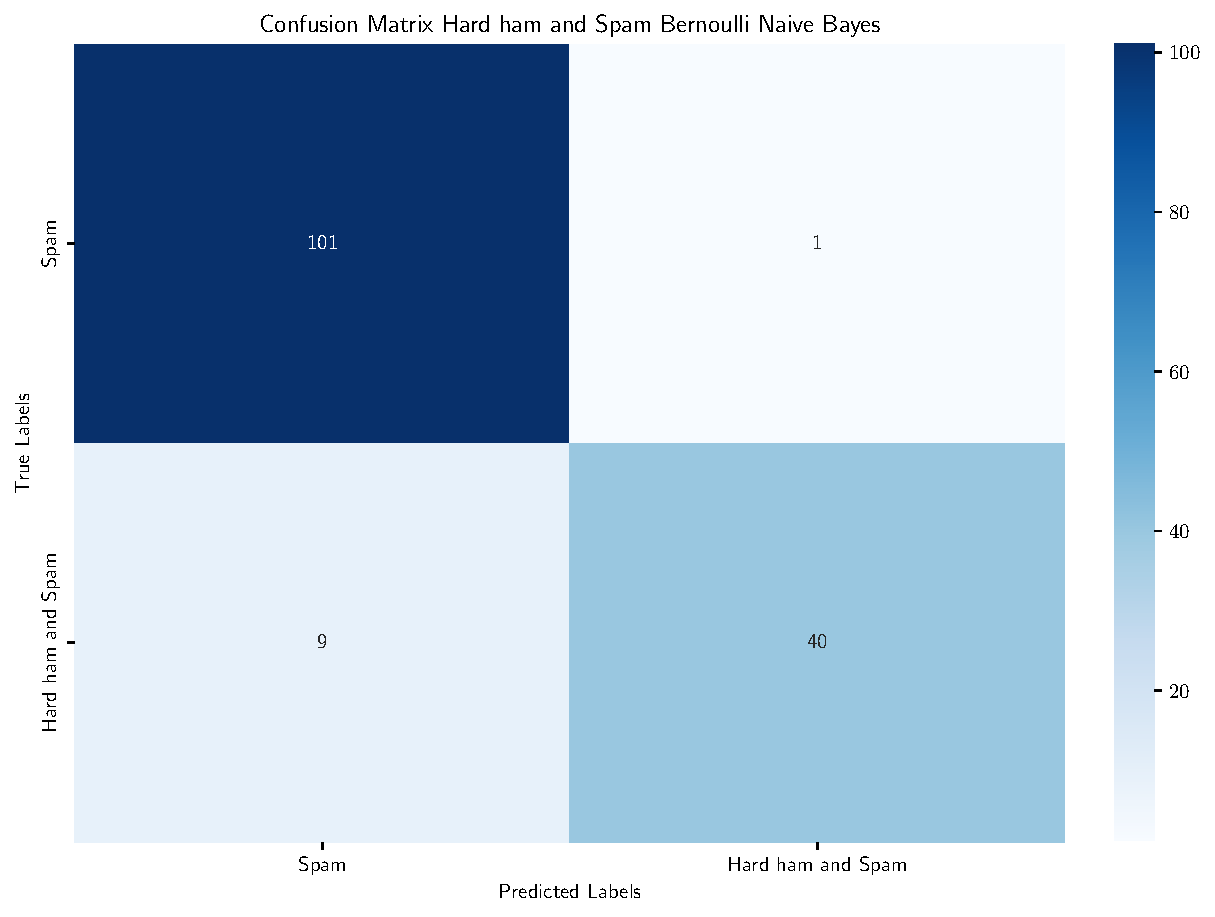
\includegraphics[width=\textwidth]{hard_ham_and_spam_bernoulli_naive_bayes_confusion_matrix.pdf}
      \caption{Hard ham vs spam, Bernoulli Naive Bayes}
      \label{fig:hard_ham_and_spam_bernoulli_naive_bayes_confusion_matrix}
  \end{subfigure}
  \vfill
  \begin{subfigure}[b]{\textwidth}
      \centering
      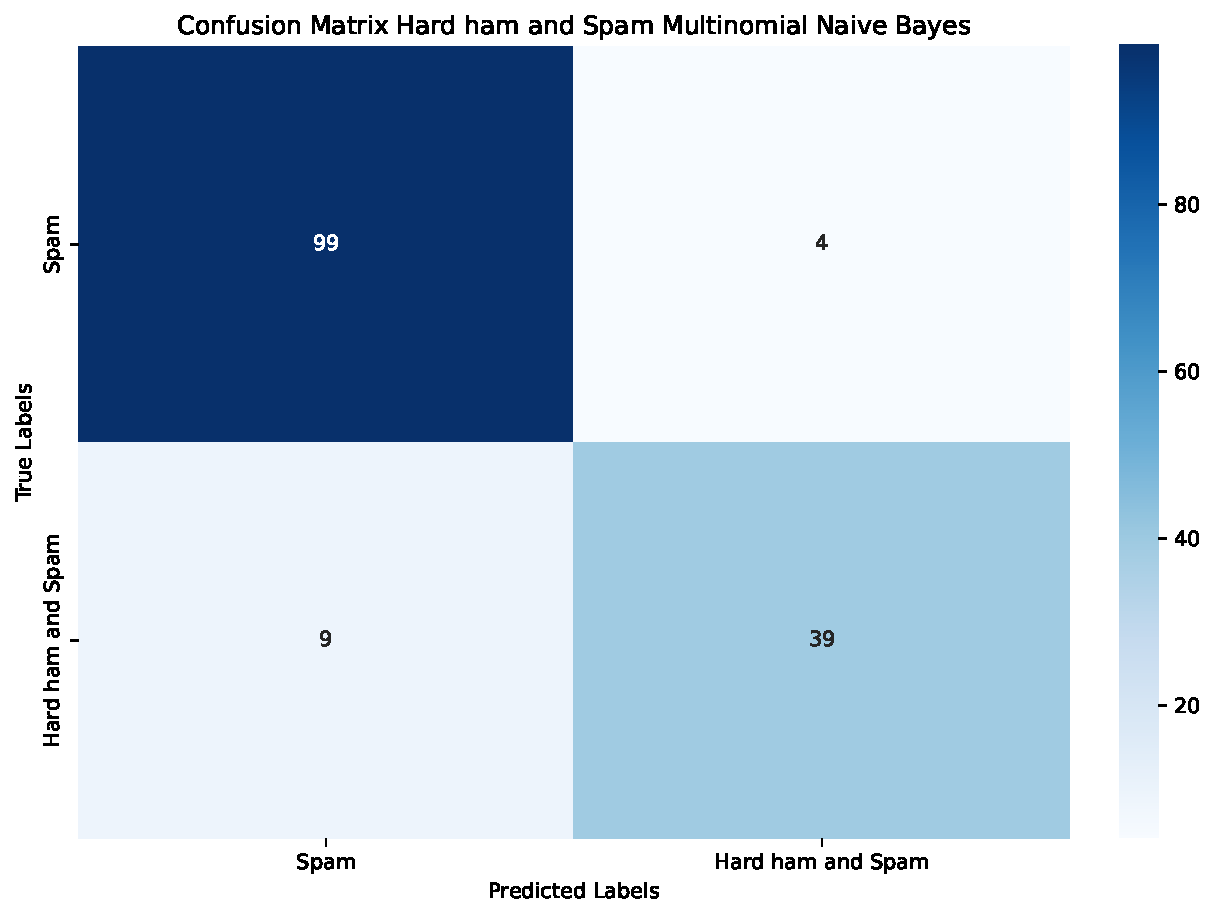
\includegraphics[width=\textwidth]{hard_ham_and_spam_multinomial_naive_bayes_confusion_matrix.pdf}
      \caption{Hard ham vs spam, Multinomial Naive Bayes}
      \label{fig:hard_ham_and_spam_multinomial_naive_bayes_confusion_matrix}
  \end{subfigure}
  \caption{Confusion matrixes of hard ham and spam}
  \label{fig:hard_ham_and_spam_confusion_matrix}
\end{figure}

\newpage





\printbibliography

\section*{Appendix: Source Code}

\lstset{
  language=Python,
  basicstyle=\ttfamily,
  commentstyle=\color{OliveGreen},
  keywordstyle=\bfseries\color{Magenta},
  stringstyle=\color{YellowOrange},
  numbers=left,
  basicstyle=\footnotesize,
  breaklines=true,
  postbreak=\mbox{\textcolor{red}{$\hookrightarrow$}\space}
}


\lstinputlisting{ola/assignment3.py}

\end{document}
